% Created 2016-05-29 Sun 12:00
\documentclass[12pt,pdftex]{article}
\usepackage[postscript]{ucs}
\usepackage[utf8x]{inputenc}
\usepackage[T1]{fontenc}
\usepackage{fixltx2e}
\usepackage{graphicx}
\usepackage{longtable}
\usepackage{float}
\usepackage{wrapfig}
\usepackage{soul}
\usepackage{textcomp}
\usepackage{marvosym}
\usepackage{amsmath}
\usepackage{wasysym}
\usepackage{latexsym}
\usepackage{amssymb}
\usepackage{amstext}
\usepackage{hyperref}
\tolerance=1000
\usepackage{pifont}
\usepackage{units}
\usepackage[a4paper,margin=20mm,top=15mm,bottom=20mm]{geometry}
\usepackage[bf,sf,small,nonindentfirst]{titlesec}
\usepackage{booktabs}
\usepackage{parskip}
\usepackage{newcent}
\usepackage{helvet}
\usepackage{pxfonts}

\renewcommand{\ttdefault}{txtt} % narrower + nicer tt font
\titleformat{\subsubsection}{\normalfont\itshape}{\thesubsubsection}{.5em}{}
\setlength{\emergencystretch}{1\textwidth} % no overfull hboxes with tt font
\usepackage{listings}
\author{Wolfgang Dobler}
\date{\today}
\title{Git Best Practises}
\hypersetup{
 pdfkeywords={},
  pdfsubject={},
  pdfcreator={Emacs 24.5.1 (Org mode 8.3beta)}}
\begin{document}

\maketitle
\tableofcontents

\thispagestyle{empty}

\begin{abstract}
\noindent%
Tips and recommendations for using Git with the Pencil code:
\begin{itemize}
\item Don't panic.
\item Never pull from the remote branch into the tracking branch.
\item Make the git history a good narrative.
\end{itemize}
\end{abstract}


\section{Operative Summary}
\label{sec-1}

Here is the bottom line of this document.

\begin{enumerate}
\item Decide whether you want to rebase or merge your local changes into
upstream (typically the \emph{origin/master} branch).

\begin{enumerate}
\item Rebase: Use '\texttt{git pull -{}-rebase}' to get upstream changes into you
local tracking branch (typically \emph{master}).

\item Merge: Do \emph{not} merge upstream into your tracking branch like this:
\lstset{frame=single,basicstyle=\ttfamily\footnotesize,language=sh,label= ,caption= ,captionpos=b,numbers=none}
\begin{lstlisting}
git pull origin/master   # DON'T!
# or
git merge origin/master  # DON'T!
\end{lstlisting}
because that breaks the SVN bridge and makes it quite difficult to
understand the history of commits.

Instead, merge your changes into upstream, either manually or
using
\lstset{frame=single,basicstyle=\ttfamily\footnotesize,language=sh,label= ,caption= ,captionpos=b,numbers=none}
\begin{lstlisting}
git pc reverse-pull  # DO THIS INSTEAD
# or
git pc reverse-merge  # DO THIS INSTEAD
\end{lstlisting}
\end{enumerate}

\item Think about using feature branches for logic units that cover more
than a few commits.

\item Don't rebase (or otherwise modify) published history.
\end{enumerate}


\section{Prerequisites}
\label{sec-2}

This text is not an introduction to Git – there are many Git tutorials
available on the web, and I will assume that you already know the basic
operations.

But for the discussion below we will need a few important concepts.

\subsection{What is Git?}
\label{sec-2-1}

Git is a flexible version-control system that is well-suited for
software development, be it with a centralized server (Github, in our
case), or in a completely decentralized setting.


\subsection{What is a Git repository?}
\label{sec-2-2}

A Git repository is a set of unique commits that form a
\href{https://en.wikipedia.org/wiki/Directed_acyclic_graph}{directed acyclic graph} (DAG) like this:
\begin{verbatim}
A---B---C---D---E---F---  master
     \     /     \
      G---H       I---J---  feature
\end{verbatim}

We say that E is a \emph{child} of D, and that D has two
\emph{parents}, C and H.
The \emph{ancestors} of D consists of A, B, C, G, and H.
The \emph{descendants} of D are E, F, I, and J.

If you know how to read this diagram, you know enough about DAGs for
our purposes.\footnote{You get extra credits if you can tell which of the commits A, E and
G belong to branch \emph{feature}.}


\subsection{What is a commit?}
\label{sec-2-3}

A commit typically represents a state of the file tree (the directory
tree you get by checking out a revision), together with its complete
commit ancestry.
So you get different commit ids (represented as hexadecimal SHA1 hash
codes) if you
\begin{itemize}
\item commit a change, commit the inverse of that change, and commit the
original change again;
\item change the commit message of your last commit (with \texttt{‘git commit
     -{}-amend’});
\item take some part of the commit graph and attach it somewhere else
(\texttt{‘git rebase’});
\item make any change to a commit that is an ancestor of the commit in
question.
\end{itemize}


\subsection{The narrative metaphor}
\label{sec-2-4}

In many respects the commit history we create with Git is a \emph{narrative}
that tells us (and others) how the code evolved to its current state.

Indeed, committing changes has a lot in common with telling a story,
and that story can be interesting or boring, it can be presented in a
logical way or totally confusing, even if the final code in both cases
is the same.

And while there are different styles of telling the story well, a badly
told narrative will make us all suffer.
So please think about the logical order in which your changes make most
sense and formulate and format your log messages appropriately.\footnote{The first line of your commit message is a \emph{heading} summarizing
what was intended, or what has happened.
The second line is traditionally kept empty, and more details can follow
on lines 3, 4, 5, etc. of the log message.}


\subsection{Atomicity}
\label{sec-2-5}

Git commands tend to be focused on one task.\footnote{One popular counter example is \texttt{‘git pull [-{}-rebase]’}, which is
pretty much just a combination of \texttt{‘git fetch’} with either \texttt{‘git merge’}
or \texttt{‘git rebase’}.}
As a consequence, what the user perceives as one logical step may
require two or three consecutive command calls.
This helps in understanding what you are doing, and when something
goes wrong you know where exactly the problem occurred.

However, if you prefer to combine several elementary git operations
into one command call (say, committing and pushing), or don't want to
type the same command-line options over and over again, you can of
course create a shell script, or you can define a \emph{Git alias}.
For example, after running
\lstset{frame=single,basicstyle=\ttfamily\footnotesize,language=sh,label= ,caption= ,captionpos=b,numbers=none}
\begin{lstlisting}
git config --global alias.where 'rev-parse --short=12 HEAD'
\end{lstlisting}
you will have a new git command ‘git where’ that tells you the SHA1
hash of the current HEAD commit.
Git aliases automatically inherit some niceties like command completion
or a \texttt{-{}-help} option.

As in other contexts, it is a virtue to not become too dependent on
such helpers, lest you forget what you are doing, have a hard time
communicating with others and feel lost in environments where those
helpers are missing.

The \emph{Pencil Code} comes with a \texttt{‘git pc’} script that provides some
combined operations.
Run \texttt{‘git pc -h’} to get a list of available sub-commands.


\section{Don't panic}
\label{sec-3}
\label{Section-dont-panic}

Or: \emph{What to do when you think you're lost}

Git will try hard to preserve your changes:

\begin{itemize}
\item Any changes you committed will be part of the \texttt{\emph{reflog}} for at least
two weeks\footnote{Unless you explicitly decide otherwise.}, even if you change or abandon them.

\item Uncommitted changes to git-controlled-files will only get overwritten
if you run one of the commands
\begin{itemize}
\item \texttt{git checkout <file-or-directory>}
\item \texttt{git reset -{}-hard}
\item And of course any non-git commands that change files
\end{itemize}

\item Files unknown to Git will only get lost with\footnote{There are corner cases where other git commands (like
\texttt{git stash -{}-include-untracked}) call \texttt{git clean}, which can in
principle \href{http://blog.icefusion.co.uk/git-stash-can-delete-ignored-files-git-stash-u/}{lead to data loss}.
However, this should only concern files that match your \texttt{.gitignore}
patterns, and if that is the case for any file you care about, you have
been asking for trouble.}
\begin{itemize}
\item \texttt{git clean}
\item Again, any non-git commands that change files
\end{itemize}
\end{itemize}


Table \ref{Table:How-to-lose-changes} summarizes this discussion.

\begin{table}[htb]
\caption{\label{Table:How-to-lose-changes}How to lose changes with git}
\centering
\begin{tabular}{ll}
\toprule
\emph{Changes} & \emph{How they can get lost}\\
\midrule
Changes committed to git & Not at all, unless you insist \footnotemark\\
\midrule
Uncommitted changes to git-controlled files & \texttt{git checkout <file-or-directory>}\\
 & \texttt{git reset -{}-hard}\\
 & Non-git commands\\
\midrule
Files unknown to Git & \texttt{git clean}\\
 & Non-git commands\\
\bottomrule
\end{tabular}
\end{table}\footnotetext[6]{Leaving important Git commits dangling (≈ unused) for more than two
weeks counts as insisting on data loss.}


\subsection{I'm almost panicking ...}
\label{sec-3-1}
\label{Section-almost-panicking}

\emph{
... for I'm afraid something got lost, although I know this is not the
case because I stayed away from the commands in Table
\ref{Table:How-to-lose-changes}.
}

\bigskip

Here is how to see almost every change\footnote{This will not show dropped stashes or stashes older than the last
one (but those are still accessible).} that was ever\footnote{Redefining “ever” = “in the last two weeks” for dangling commits.}
known to git:
\lstset{frame=single,basicstyle=\ttfamily\footnotesize,language=sh,label= ,caption= ,captionpos=b,numbers=none}
\begin{lstlisting}
gitk --reflog --all
# or
tig --reflog --all
# or, without graphics,
git reflog --all --glob='stash*'

# If you prefer melodramatic command names, try
git pc panic
\end{lstlisting}

If you want to also see dropped stashes, you can use
\lstset{frame=single,basicstyle=\ttfamily\footnotesize,language=sh,label= ,caption= ,captionpos=b,numbers=none}
\begin{lstlisting}
git pc panic --full
\end{lstlisting}


\section{Joining different lines of development}
\label{sec-4}
\label{Section:Joining-lines-of-development}

In a community coding project like the \emph{Pencil Code}, we will
frequently have a situation like this:
\begin{verbatim}
A---B---C-----  branch1
     \
      F---G---  branch2
\end{verbatim}
where different (diverging) commits have been made on different
branches (very often, these branches are the remote branch
\emph{origin/master} and the local tracking branch \emph{master}), and we want to
integrate both lines of development into one.

Git offers two different techniques to achieve that goal: \emph{merging} and
\emph{rebasing}.
Tobias Heinemann has created a screencast where he
\href{https://asciinema.org/a/dauj562l4uwr7bpyohqyewkj5}{demonstrates different variants of these approaches}.


\subsection{What is merging?}
\label{sec-4-1}
\label{Merge}

A \emph{merge} commit adds a new connection to parts of the Git graph.
For example, if we have the following situation
\begin{verbatim}
A---B---C-----  master
     \
      F---G---  feature
\end{verbatim}
and want to bring the changes from branch \emph{feature} to \emph{master}, we
can merge \emph{feature} into \emph{master} and get
\begin{verbatim}
A---B---C---D---  master
     \     /
      F---G-----  feature
\end{verbatim}

In the pure DAG sense, the two parents C and G of the merge commit D
are completely equivalent, but for reasons discussed \texttt{below}, we want to
make sure we merge \emph{feature} into \emph{master} (so C is the \emph{first parent}
and G is the \emph{second parent}), not the other way around.

You remember our narrative metaphor?
If you always \emph{merge} your commits or groups of commits because you
don't want to modify history, you are narrating in a diary or
chronicler's style.


\subsection{What is rebasing?}
\label{sec-4-2}
\label{Rebase}

In the example above, we have a second option to bring the feature
branch's changes into master, by creating new commits that contain
those changes, but start from the state C, not B:
\begin{verbatim}
A---B---C-----------  master
         \
          F'---G'---  feature
\end{verbatim}
We say that we have \emph{rebased} the commits F and G from B onto C.

Rebasing modifies history, which is only permissible as long as this
history is \emph{local}.
So \emph{don't rebase published commits}.
The commits that are eligible to rebasing are the ones displayed by
\lstset{frame=single,basicstyle=\ttfamily\footnotesize,language=sh,label= ,caption= ,captionpos=b,numbers=none}
\begin{lstlisting}
gitk origin/master..master
# or
tig origin/master..master
# or, without graphics,
git log origin/master..master
\end{lstlisting}

Even if the new commit F' may introduce the same textual
difference as the original commit F, the file-tree state it represents
is completely new and there is no guarantee that it will e.g.~compile,
even if both, C and F do.

Once you finish the rebase, you appear to have lost the original change
F by pretending that you were applying a change F' in the first
place.\footnote{This is of course not true: you can use \texttt{‘git reflog’} and friends
to view your original changes, see
Sec.~\ref{Section-almost-panicking}.}
That's perfectly OK, as you will no longer be interested in the
original change when the new version gets part of the Git narrative.


\bigskip

Rebasing is not an exclusive option.
Even if you routinely rebase your local changes, you will want to
merge longer-lived feature branches.

In terms of narrating, \emph{rebasing} allows you to use letter style, where
you bring facts into logical frames and order them accordingly (because
nobody would want to read your stream-of-consciousness letters).


\subsection{Pros and cons}
\label{sec-4-3}

Here is the decision matrix for merging vs. rebasing

\begin{center}
\begin{tabular}{lll}
\toprule
Criterion & Merge & Rebase\\
\midrule
Resulting graph structure & More complex & Simpler\\
History & Preserved & Modified\\
Safety & Safer & Less safe \footnotemark\\
\bottomrule
\end{tabular}
\end{center}\footnotetext[10]{Less safe in the sense that conflicts can put you in a
detached-head state.}

In short, use merging when you are afraid – but you know from
Sec.~\ref{Section-dont-panic} that you needn't be afraid.


\subsubsection{Graph structure}
\label{sec-4-3-1}

Every merge commit increases the connectivity of the commit graph by
one\footnote{Or even more than one, in the case of an \emph{octopus merge}.
But those are somewhat exotic.}.
A rebase, by contrast, does not change the connectivity and leads to a
more linear history.


\subsubsection{The worst thing that can happen}
\label{sec-4-3-2}

If you have conflicts, rebasing can bring your working-directory into
a state where you are not on any branch (\emph{detached head}).
This is not really something to worry about:
Just fix the conflicts, \texttt{‘git add’} the changes, and do \texttt{‘git rebase
    -{}-continue’} to finish the rebase; and in case you get lost, do \texttt{‘git
    rebase -{}-abort’} and start afresh.
Even if you get completely lost and resort to measures like
\texttt{‘git reset’}, \hyperref[sec-3]{you needn't be afraid} to lose history.


\section{Best practices}
\label{sec-5}

\subsection{Don't merge upstream into your tracking branch}
\label{sec-5-1}
\label{S-developing-on-master}

Suppose you just started developing code on \emph{master}.
Your branches look like this (A and B are commits, the `o' is just
a visual connector):
\begin{verbatim}
--A---B-----  origin/master (remote branch)
       \
        o---  master (local tracking branch)
\end{verbatim}


\bigskip

Despite its name, the \emph{remote branch} exists only on your computer.
It represents what is known about a branch called \emph{master} on the
server and serves for synchronization with the server.
You cannot directly commit to this branch.

The tracking branch reflects how you would like the server branch to
look like.\footnote{And if that is not compatible with the server's latest history, you
modify the tracking branch until it is.}


\bigskip


Now you commit some changes X, Y to your local tracking branch:
\begin{verbatim}
--A---B----------  origin/master
       \
        X---Y----  master
\end{verbatim}
and want to push them to the server.
If the server is still at commit B, this will result in
\begin{verbatim}
--A---B---X---Y-----  origin/master
               \
                o---  master
\end{verbatim}
and you are done.

However, if somebody has committed changes to the server before you
push, you will get an error message\footnote{Do you see the ellipses in the
suggested \texttt{'git pull ...'} command? Git did \emph{not} say you should
run just \texttt{‘git pull’} without any arguments. If you accidentally
\emph{do} happen to run \texttt{'git pull'} without arguments, then you can
undo this by running \texttt{'git reset -{}-merge HEAD$\sim$1'}}:

{\small
\begin{verbatim}
To [...]
 ! [rejected]        master -> master (fetch first)
error: failed to push some refs to [...]
hint: Updates were rejected because the remote contains work that you do
hint: not have locally. This is usually caused by another repository pushing
hint: to the same ref. You may want to first integrate the remote changes
hint: (e.g., 'git pull ...') before pushing again.
hint: See the 'Note about fast-forwards' in 'git push --help' for details.
\end{verbatim}
}

Before you can fix the problem, you need to \texttt{‘git fetch’} to update the
remote branch:
\begin{verbatim}
--A---B---C---D---E---  origin/master
       \
        X---Y---------  master
\end{verbatim}

Now your task is to bring the two lines of development together, and
you can either do this \hyperref[Rebase]{using rebase}, or \hyperref[Merge]{using merge}.


\subsubsection{Alternative 1: Rebase}
\label{sec-5-1-1}

Rebasing is straight-forward, you run\footnote{If you have uncommitted changes
at this point, Git will refuse to do anything before you have stashed them
away. Git can do this for you automatically if you run
\texttt{'git rebase --autostash origin/master'} instead. See footnote
\ref{fn:autostash} for more information on Git's \texttt{'autostash'}
functionality.}
\lstset{frame=single,basicstyle=\ttfamily\footnotesize,language=sh,label= ,caption= ,captionpos=b,numbers=none}
\begin{lstlisting}
git rebase origin/master
\end{lstlisting}
if necessary deal with conflicts (that will temporarily throw your
repository into a headless state) and end up with
\begin{verbatim}
--A---B---C---D---E-----------  origin/master
                   \
                    X'---Y'---  master
\end{verbatim}
You have changed your commits by turning them into descendants of E (and
possibly by including solutions for conflicts) and you can now push to
get
\begin{verbatim}
--A---B---C---D---E---X'---Y'----  origin/master
                            \
                             o---  master
\end{verbatim}
As mentioned earlier, this approach gives you a linear history similar
to what you know from \emph{Subversion}.

\bigskip

While it is completely feasible to first fetch, then rebase, you can
have both in one command:
\lstset{frame=single,basicstyle=\ttfamily\footnotesize,language=sh,label= ,caption= ,captionpos=b,numbers=none}
\begin{lstlisting}
git pull --rebase
\end{lstlisting}
This is equivalent to \verb~git fetch; git rebase origin/master~, so it is
exactly what we need\footnote{You can even set the \texttt{-{}-rebase} option via your git configuration,
using\\
\noindent\qquad\qquad  \texttt{git config -{}-global branch.master.rebase true}\\
\noindent\qquad\qquad  \texttt{git config -{}-global branch.autoSetupRebase always}\\
and henceforth when you type \texttt{‘git pull’}, you will in fact do
\texttt{‘git pull -{}-rebase’}.

However, tacitly changing the behaviour of commands is a great source of
confusion.
Sooner or later you will work on a system where you have not set these
flags (e.g. because you forgot, or you are helping somebody else).
Without thinking twice, you will type \texttt{‘git pull’}, then \texttt{‘git push’},
and, voilà: after half year of disciplined commits by everybody, you
managed to break the SVN bridge again.

Thus, it is better to just get into the habit of always using \texttt{git pull}
with the \texttt{-{}-rebase} flag.}

\bigskip

To summarize this subsection:
To push your committed changes, run
\lstset{frame=single,basicstyle=\ttfamily\footnotesize,language=sh,label= ,caption= ,captionpos=b,numbers=none}
\begin{lstlisting}
git pull --rebase
# [test]
git push
\end{lstlisting}
and life will be beautiful.\footnote{If you happen to have uncommitted changes when you want to
\texttt{‘git pull -{}-rebase’}, Git will refuse to do anything before you have
stashed them away.
With Git \(\ge\) 2.6, you can configure \verb~rebase.autostash=true~ to have git
automatically stash away your uncommitted changes and restore them after
the pull.
For older versions of Git, you get the same functionality with
\texttt{‘git pc pull-and-rebase’}, i.e.\\
\noindent\qquad\qquad  \texttt{git pc pull-and-rebase}\\
\noindent\qquad\qquad  \texttt{\# [test]}\\
\noindent\qquad\qquad  \texttt{git push}\label{fn:autostash}}


\subsubsection{Alternative 2: Merge the other way around}
\label{sec-5-1-2}

Alternatively, we \emph{can} merge the two branches together.
Here the discussion gets more complicated, so we moved it
to Appendix \ref{Section-which-way-to-merge}.

The take-home message is to merge not the remote branch into the
tracking branch:
\lstset{frame=single,basicstyle=\ttfamily\footnotesize,language=sh,label= ,caption= ,captionpos=b,numbers=none}
\begin{lstlisting}
git pull origin/master   # DON'T DO THIS
# or
git merge origin/master  # DON'T DO THIS
\end{lstlisting}
but rather the other way around, because
\emph{%
the commit you push must not be a merge of \emph{origin/master} into
\emph{master}.
}

Getting this right typically involves some temporary branch or tag and
a \texttt{git reset}, but as an alternative, you can use our
\lstset{frame=single,basicstyle=\ttfamily\footnotesize,language=sh,label= ,caption= ,captionpos=b,numbers=none}
\begin{lstlisting}
git pc reverse-pull origin/master   # DO THIS INSTEAD
# or
git pc reverse-merge origin/master  # DO THIS INSTEAD
\end{lstlisting}

\bigskip

The higher-level rule behind this is as follows:
\begin{quote}
\setlength{\fboxsep}{8pt}
\fbox{%
\begin{minipage}{0.7\textwidth}%
\slshape
\textbf{Rule 1:}
The first-parent history of \emph{origin/master} should correspond to the
order in which the commits appeared on the server and may thus only be
appended to.
\end{minipage}%
}
\end{quote}

If you violate this rule, you pretend that changes that were already on
the server have only just appeared there due to your merge, and that
your changes have been on the server before.
As a consequence, tools like the GitHub SVN bridge or the commit emails
will fail, and history will generally become misleading.

See Appendix \ref{Section-which-way-to-merge} for a discussion of
\emph{first-parent} history.


\subsection{Feature branches}
\label{sec-5-2}

\begin{itemize}
\item When you are working on one topic and expect more than a
handful\footnote{Even just two or three commits may be enough to go for a feature
branch if that improves the narrative.} of changes, consider using a \emph{feature branch}.

\item When you are collaborating on a topic with somebody else and your
changes are not yet ready for the others, use a feature branch.
\end{itemize}


To work with a feature branch, just go to the latest commit of \emph{master}
(the later you start the branch, the fewer conflicts you will create),

\lstset{frame=single,basicstyle=\ttfamily\footnotesize,language=sh,label= ,caption= ,captionpos=b,numbers=none}
\begin{lstlisting}
git checkout master
git pull --rebase
\end{lstlisting}
and create the branch
\lstset{frame=single,basicstyle=\ttfamily\footnotesize,language=sh,label= ,caption= ,captionpos=b,numbers=none}
\begin{lstlisting}
git checkout -b cool-new-feature
\end{lstlisting}

\bigskip

If that branch is long-lived, you will want to occasionally merge
\emph{master} into it.\footnote{This does \emph{not} violate our rule
`\hyperref[sec-5-1]{don't merge upstream into your local tracking branch}'.}
Say, you have this situation
\begin{verbatim}
--A---B---C---D---E---  master
   \
    N---O---P---Q-----  feature
\end{verbatim}
Run
\lstset{frame=single,basicstyle=\ttfamily\footnotesize,language=sh,label= ,caption= ,captionpos=b,numbers=none}
\begin{lstlisting}
git fetch origin  #  update origin/master from the server
git stash         # if you have uncommitted local changes
\end{lstlisting}

Then do
\lstset{frame=single,basicstyle=\ttfamily\footnotesize,language=sh,label= ,caption= ,captionpos=b,numbers=none}
\begin{lstlisting}
git checkout master            # check out your local tracking branch ...
git pull --rebase              # ... and bring it up to date

git checkout cool-new-feature  # go back to your feature branch
git merge master               # do the actual merge
\end{lstlisting}
to obtain
\begin{verbatim}
--A---B---C---D---E-----  master
   \               \
    N---O---P---Q---R---  feature
\end{verbatim}


There are some shorter variants to this procedure. You can use our
\texttt{‘git pc’} script like this:
\lstset{frame=single,basicstyle=\ttfamily\footnotesize,language=sh,label= ,caption= ,captionpos=b,numbers=none}
\begin{lstlisting}
git fetch origin  #  update origin/master from the server
git pc ff-update master  # update master without checking it out
git merge master         # do the actual merge
\end{lstlisting}
or you could directly merge the remote branch
\lstset{frame=single,basicstyle=\ttfamily\footnotesize,language=sh,label= ,caption= ,captionpos=b,numbers=none}
\begin{lstlisting}
git merge origin/master
\end{lstlisting}
although this is less common than merging the local tracking branch.

After merging, don't forget to
\lstset{frame=single,basicstyle=\ttfamily\footnotesize,language=sh,label= ,caption= ,captionpos=b,numbers=none}
\begin{lstlisting}
git stash pop
\end{lstlisting}
if you have stashed changes before you merged.

\bigskip

When your branch is ready for merging back, you do
\lstset{frame=single,basicstyle=\ttfamily\footnotesize,language=sh,label= ,caption= ,captionpos=b,numbers=none}
\begin{lstlisting}
git checkout master
git pull --rebase           # bring master up-to-date
git merge cool-new-feature
[test]
git push
\end{lstlisting}

The topology now looks like this:
\begin{verbatim}
--A---B---C---D---E---F---G---H---I--- master
   \               \             /
    N---O---P---Q---R---S---T---U      feature
\end{verbatim}

\bigskip

What if that push failed due to somebody committing new changes
upstream?

No problem.
We tag the first merge attempt and merge that tag to the updated
upstream branch:
\lstset{frame=single,basicstyle=\ttfamily\footnotesize,language=sh,label= ,caption= ,captionpos=b,numbers=none}
\begin{lstlisting}
# remember, we are on master
git push   # fails: "! [rejected] master -> master (fetch first)"

git tag previous-merge-of-cool-new-feature
git fetch                       # update origin/master
git reset --hard origin/master  # update local master branch
git merge previous-merge-of-cool-new-feature
[test]
git push
\end{lstlisting}

The narrative now says:
We have tried to merge \emph{cool-new-feature} into master, but failed to
push that, so we then merged that first merge into master and pushed.
That may be more detail than we wanted (and more steps than we
anticipated), but describes exactly what happened:

\begin{verbatim}
--A---B---C---D---E----F-----G----H---X---Y--- master
   \               \               \     /
    \               \               I---o
     \               \             /
      N---O---P---Q---R---S---T---U            feature
\end{verbatim}


\bigskip


Using \emph{feature branches} with appropriate granularity, you tell the
story in a kind of novelist style.
Actually, the metaphor falls short in this case, as your audience has
the choice to read just a synopsis (by looking at the main branch only)
or go into small details (reading the commits inside the feature
branches).


\appendix



\section{Which way to merge}
\label{sec-6}
\label{Section-which-way-to-merge}

Consider the situation from Sec. \ref{S-developing-on-master}, where
you want to join your line of development with what happened on the
server:
\begin{verbatim}
--A---B---C---D---E--  origin/master
       \
        X---Y--------  master
\end{verbatim}

It is tempting to just call
\lstset{frame=single,basicstyle=\ttfamily\footnotesize,language=sh,label= ,caption= ,captionpos=b,numbers=none}
\begin{lstlisting}
git pull                 # DON'T DO THIS
# or, equivalently,
git fetch
git merge origin/master  # DON'T DO THIS
\end{lstlisting}
which would give you the following repository structure
\begin{verbatim}
--A---B---C---D---E-----  origin/master
       \           \
        X-----Y-----M---  master
\end{verbatim}
This doesn't look bad, so you now push \emph{master} to the server and get
\begin{verbatim}
--A---B---C---D---E---M-----  origin/master
       \             / \
        X-----------Y   o---  master
\end{verbatim}

Topologically, that is exactly what we want.
But there is more to a git repository than pure topology of the
directed acyclic graph: there is an order in parentage.
Y is the \emph{first parent} of the merge commit M, while E is the \emph{second
parent}:\footnote{My notation in the graph is adopted from
\href{http://git-blame.blogspot.de/2015/03/fun-with-non-fast-forward.html}{Junio Hamano's Blog}.
Another good discussion on the importance of first-parent history can
be found on the \href{http://devblog.nestoria.com/post/98892582763/maintaining-a-consistent-linear-history-for-git}{Nestoria Dev Blog}.}
\begin{verbatim}
                    2
--A---B---C---D---E---M-----  origin/master
       \             /1\
        X-----------Y   o---  master
\end{verbatim}

Straightening out the first-parent connection, this can be rearranged as
\begin{verbatim}
                1
--A---B---X---Y---M-----  origin/master
       \         /2 \
        C---D---E   o---  master
\end{verbatim}
and indeed this is what many tools will show you.\footnote{Including the \href{https://github.com/pencil-code/pencil-code/network}{GitHub network graph}, gitk (to some extent) and the
GitHub SVN bridge.}

For example, commands like \texttt{gitk -{}-first-parent} (or simply \texttt{git log
  -{}-first-parent}), give
\begin{verbatim}
--A---B---X---Y---M-----  origin/master
           \     / \
                    o---  master
\end{verbatim}
which suggests that the main chain (= first-parent lineage) of commits
on the server has disruptively changed from
\begin{verbatim}
--A---B---C---D---E-----
\end{verbatim}
to
\begin{verbatim}
--A---B---X---Y---M-----
\end{verbatim}

If the SVN bridge has to rely on first-parent lineage between commits to
create its linear history, such a reinterpretation leads to a new SVN
repository structure that is not compatible with what we had before.
Hence, it is not surprising that such merges cause troubles with the SVN
bridge:
\begin{verbatim}
$ svn commit <file>
svn: E160024: Transmission failed (Details follow):
svn: E160024: resource out of date; try updating
\end{verbatim}


\bigskip

So is it really wrong to merge?
Not if you merge the right way around.
You need to create a merge commit where the latest upstream commit (E
in our example) is the \emph{first parent}, and the tracking-branch commit
(Y) is the \emph{second parent}.

How to do this is left as an exercise to the reader.
It is not very tricky, but for convenience we have a \texttt{git-pc} command
\lstset{frame=single,basicstyle=\ttfamily\footnotesize,language=sh,label= ,caption= ,captionpos=b,numbers=none}
\begin{lstlisting}
git pc reverse-pull origin/master   # DO THIS INSTEAD
# or
git fetch
git pc reverse-merge origin/master  # DO THIS INSTEAD
\end{lstlisting}
that gives you exactly the desired structure:
\begin{verbatim}
                    1
--A---B---C---D---E---M-----  origin/master
       \             /2\
        X-----------Y   o---  master
\end{verbatim}
which you can push without violating our Rule 1.

\bigskip

Apart from avoiding problems with the SVN bridge, merging the right way
around will also lead to a much more meaningful history.
Consider the following real-life example:\footnote{The output was obtained using \texttt{tig} on the Pencil Code repository,
removing many commits, shortening and mildly anonymizing the commits.}

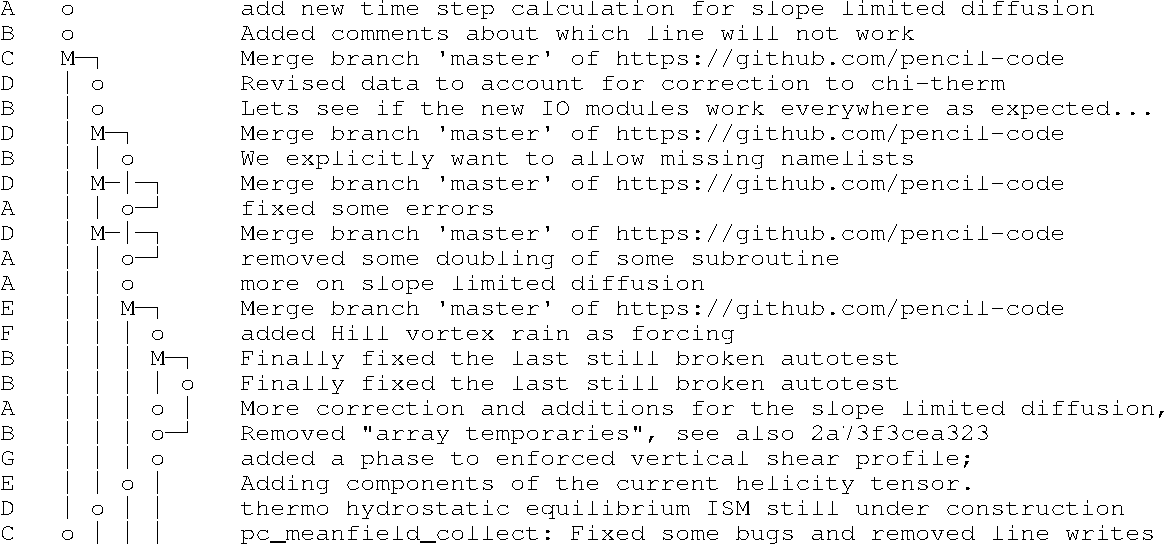
\includegraphics[width=.97\linewidth]{git-wrong-history.pdf}

So, did users A, B and G really work on the same feature branch to add
phase to the shear profile, remove array temporaries and to correct
slope limited diffusion?
And did those commits get merged in a commit that claims to have fixed
the last broken autotest?

The true story must have been more like this:

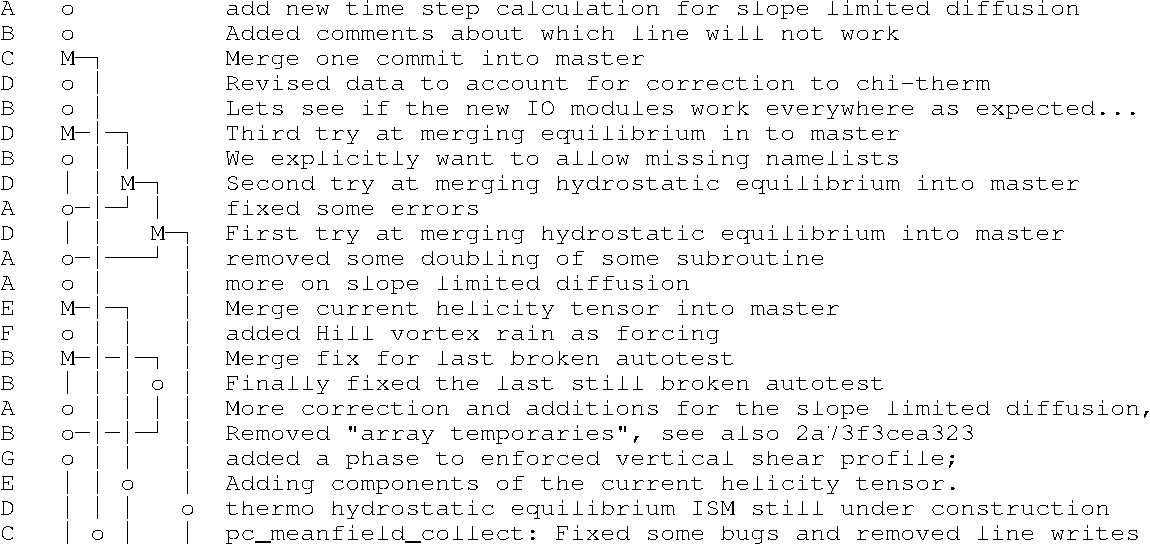
\includegraphics[width=.97\linewidth]{git-better-history.pdf}

Most of the development happened on the main line, but occasionally
somebody had a change that needed to get merged into that line, because
other commits got pushed first.

And indeed something like this is how \texttt{tig} would have drawn the graph,
had all of the merges been from tracking branch into the remote branch
and not the other way around.
% Emacs 24.5.1 (Org mode 8.3beta)
\end{document}
